% paper/stopless/main.tex — StoplessGC: capability revocation as the read
% barrier of a moving Java GC on CHERI/Morello.
%
% Build: make (uses the texlive/texlive docker image).
% Figures: python3 plots.py (regenerates figs/*.pdf from ../data).
%
% EVIDENCE DISCIPLINE: every number in §6 comes from paper/data/*.txt in
% this repository; every literature claim was verified against the cited
% publication on 2026-06-12 (see refs.bib header).

\documentclass[acmsmall,nonacm,screen]{acmart}

\usepackage{booktabs}
\usepackage{listings}
\usepackage{xcolor}
\usepackage{tikz}
\usetikzlibrary{arrows.meta,positioning}

\lstset{
  basicstyle=\ttfamily\small,
  breaklines=true,
  columns=fullflexible,
  keepspaces=true,
}

\title{Trap, Forward, Resume: Capability Revocation as the Read Barrier
       of a Moving Garbage Collector on CHERI}

\author{Xiaohui Luo}
\authornote{The system and this manuscript were produced by Claude
(Anthropic)---Opus~4.8 and Fable~5 models, via Claude Code---working
autonomously under the direction and review of the human author, who
takes full responsibility for the content. Current publisher and arXiv
policies do not permit listing an AI system as an author; this note and
the statement at the end of the paper are the prominent disclosure those
policies require.}
\affiliation{\institution{Independent Researcher}\country{China}}
\email{lmhtq1991@gmail.com}

\begin{abstract}
Concurrent moving garbage collectors pay for relocation with a read
barrier: a check on reference loads that redirects stale references to
relocated objects. Production collectors implement the barrier in
software---ZGC's colored-pointer test, Shenandoah's forwarding
pointer---or, in one famous case, in custom silicon. CHERI capability
hardware offers a commodity-adjacent alternative that has not been
exploited: \emph{capability revocation}, designed for C/C++ temporal
memory safety, makes the load--store unit itself fault on any use of a
revoked pointer. We repurpose this safety mechanism as a moving
collector's read barrier. Our collector, StoplessGC, relocates objects,
revokes the capabilities to the old copies, and lets the hardware trap
each surviving stale reference; a signal handler forwards the faulting
register through a forwarding table and resumes the load. No check is
executed on the hot path of reference loads---the barrier is the MMU's
tag check, which purecap code pays anyway.

We implement StoplessGC in the OpenJDK~17 template interpreter on Arm
Morello (pure-capability CheriBSD) and measure it under QEMU system
emulation. The relocation pause is bounded by the root-set size and is
independent of heap size: with the root set held constant, the pause
varies by 6\% while the live heap grows $46\times$. The dominant cost is
the whole-address-space revocation sweep, which is linear in memory
size; because the sweep cost is independent of how many objects it
revokes, batching relocations across collection cycles amortises the
mean cycle pause by $11.9\times$ without breaking our integrity tests.
We also report the design points that capability hardware forces on a
moving collector---most notably that forwarding metadata must not be
stored as capabilities, since the revocation sweep destroys the
collector's own state---and a taxonomy of the pure-capability porting
hazards we hit in HotSpot.
\end{abstract}

\begin{document}
\maketitle

% =====================================================================
\section{Introduction}
\label{sec:intro}

A moving garbage collector must ensure that no mutator dereferences a
stale reference to an object that has been relocated. Concurrent
collectors enforce this with a \emph{read barrier}~\cite{baker78}:
extra work on reference loads that detects stale references and
redirects them. The engineering history of low-latency Java collectors
is largely a history of making this barrier cheap. Azul's Pauseless
collector put it in custom hardware~\cite{pauseless}; C4 re-implemented
it in software on x86~\cite{c4}; Shenandoah dereferences a per-object
forwarding pointer~\cite{shenandoah,brooks84}; ZGC tests metadata bits
embedded in the pointer itself~\cite{zgc-toplas}. In every case the
mutator executes instructions on the hot path of reference loads that
exist only for the collector's benefit.

CHERI~\cite{cheri-isa-v9} and its Arm Morello
implementation~\cite{morello-platform} change the substrate. In
pure-capability (``purecap'') code, every pointer is a 128-bit
capability with hardware-checked bounds, permissions, and an
out-of-band validity tag; every load and store is checked by the
load--store unit at no software cost. On top of this, CheriBSD provides
\emph{capability revocation}~\cite{cherivoke,cornucopia}: mark an
address range in a shadow bitmap, and a kernel sweep atomically
invalidates every capability in the address space that points into the
marked range. Subsequent use of a revoked capability traps. Revocation
was designed to give C and C++ heaps temporal memory safety---to make
use-after-free fail-stop---and its costs and mechanisms have been
studied in that setting~\cite{cherivoke,cornucopia,cornucopia-reloaded}.

Our observation is that revocation is, almost verbatim, the read
barrier of a moving collector. The difference is what happens at the
trap. In the temporal-safety setting a revoked capability is a
use-after-free; the program is wrong and stops. In a moving collector a
revoked capability is merely \emph{stale}; the object lives on at a new
address. If the trap handler can map the old address to the new object,
it can repair the faulting register and resume the load. The hardware
provides exact, per-capability staleness detection on every dereference;
the collector only pays, lazily, for references that are actually used.

We built this collector. StoplessGC\footnote{The name is an homage to,
not a claim of lineage from, the Stopless real-time collector of Pizlo
et al.~\cite{pizlo-stopless}, which addresses lock-free concurrent
compaction on conventional hardware.} relocates Java objects with a
capability-preserving copy, records \emph{from}$\to$\emph{to} in a
forwarding table, revokes the old copies, and heals each trapped
mutator access in a \texttt{SIGPROT} handler. To our knowledge it is
the first garbage collector to use capability revocation as the read
barrier of a moving collector---prior CHERI revocation work invalidates
pointers but never forwards them, and prior Java-on-CHERI work ports
only non-moving or stop-the-world-compacting
collectors~\cite{mojo-jvm}.

This paper makes the following contributions:
\begin{itemize}
\item \textbf{Mechanism} (\S\ref{sec:design}): the
  trap--forward--resume protocol; an identity barrier for reference
  equality, the one operation that must observe relocation but does not
  dereference; and batched revocation, which exploits the fact that the
  sweep's cost is independent of the number of objects revoked.
\item \textbf{A capability-specific design law}
  (\S\ref{sec:design:fwd}): the collector's forwarding metadata must be
  stored as plain integers, not capabilities. The revocation sweep
  scans \emph{all} memory---including the collector's own tables---and
  will destroy forwarding entries that point into ranges revoked by a
  later cycle. We learned this from a corruption bug whose signature we
  describe so others can recognise it.
\item \textbf{Implementation} (\S\ref{sec:impl}): StoplessGC in the
  OpenJDK~17 template interpreter on purecap CheriBSD/Morello,
  $\sim$2.6\,kLOC of new runtime plus interpreter patches, with a
  taxonomy of the purecap porting hazards that cost us the most time.
\item \textbf{Measurement} (\S\ref{sec:eval}): with the root set held
  constant, the relocation pause varies 6\% while the live heap grows
  $46\times$ ($3.6\to163$\,MiB)---the pause is bound to roots, not heap.
  The revocation sweep is linear in memory size and dominates total
  cost; batching amortises the mean cycle pause $11.9\times$ at batch
  size 32. Healing a trapped reference costs $\sim$9\,\textmu s under
  emulation, and the identity barrier's slow path executes only
  hundreds of times per run.
\end{itemize}

We are explicit about scope (\S\ref{sec:limits}): the evaluation runs
under QEMU system emulation, so absolute times are inflated and only
the \emph{shapes}---flat versus linear, the amortisation ratio---are
architectural claims; relocation is stop-the-world in the measured
configuration (a concurrent collector thread is implemented and stable
under light load); and execution is interpreter-only, as JIT
compilation on Morello remains future work across the ecosystem.

% =====================================================================
\section{Background}
\label{sec:bg}

\subsection{CHERI, Morello, and purecap execution}

A CHERI capability is a 128-bit pointer carrying a 64-bit address,
compressed bounds, permissions, and a 1-bit validity tag held
out-of-band by the memory subsystem~\cite{cheri-isa-v9}. Capabilities
can only be derived from other capabilities by monotonic restriction
(narrow the bounds, drop permissions); any attempt to forge or widen
one clears the tag, and dereferencing an untagged capability traps. In
purecap code every pointer---every Java object reference included---is
a capability, and ordinary loads and stores are capability-checked by
hardware. Morello~\cite{morello-platform} is Arm's experimental
implementation; CheriBSD~\cite{cheribsd} is the FreeBSD-derived OS that
runs purecap userspace.

\subsection{Capability revocation}

Revocation gives CHERI heaps temporal safety.
CHERIvoke~\cite{cherivoke} established the sweeping-revocation design:
quarantine freed memory, mark it in a shadow bitmap, then sweep memory
and clear the tag of (or strip the permissions of, depending on kernel
build) every capability pointing into marked ranges.
Cornucopia~\cite{cornucopia} implemented this in CheriBSD with kernel
support, and Cornucopia Reloaded~\cite{cornucopia-reloaded} nearly
eliminated its stop-the-world pauses using Morello's per-page
capability-load generation barrier. CheriBSD exposes the mechanism to
userspace as a shadow bitmap plus a \texttt{cheri\_revoke} system call.
Throughout this line of work the post-revocation trap is a
\emph{verdict}---the access is a temporal-safety violation. No
forwarding is needed because freed objects have no successor.

\subsection{Read barriers in moving collectors}

Baker's incremental collector~\cite{baker78} introduced the read
barrier; Brooks~\cite{brooks84} made it an unconditional indirection
through a forwarding pointer. Appel, Ellis, and
Li~\cite{appel-ellis-li} moved the check into hardware a generation
early, using virtual-memory page protection: protect from-space pages
and let the fault handler evacuate. Its granularity problem---one
page-sized fault stalls every object on the page, and protection
changes require TLB shootdowns---foreshadows our per-capability
contrast. Azul's Pauseless collector~\cite{pauseless} added a dedicated
read-barrier instruction to the Vega processor; C4~\cite{c4} brought
the same loaded-value-barrier design to x86 in software. ZGC encodes
GC state in unused high bits of the 64-bit pointer (``colored
pointers'') and tests them on load, using multiple virtual mappings of
the heap to make the colored address dereferenceable~\cite{zgc-toplas}.
Shenandoah~\cite{shenandoah} stores a forwarding pointer in the object
header.

\subsection{Java on CHERI, and why ZGC's encoding does not transfer}
\label{sec:bg:zgc}

The MOJO project ported OpenJDK~17 to purecap CheriBSD/Morello,
including the Epsilon, Serial, and G1 collectors~\cite{mojo-jvm}; the
concurrent moving collectors (ZGC, Shenandoah) were not ported. This is
not an accident of effort: ZGC's two structural optimisations are
specifically hostile to capabilities. Colored pointers require unused,
software-controlled address bits, but a capability's address must stay
within its bounds and cannot carry out-of-band metadata---and the
pointer is 128 bits with a hardware-owned tag, so ``just use the high
bits'' forges an invalid capability. Multi-mapping requires the same
physical object to be reachable at several virtual addresses, but a
capability is bound to the address range it was derived for;
dereferencing the same object through a differently-colored alias
requires re-deriving capabilities at every color flip. A
capability-native moving collector needs a different barrier
mechanism, which is what this paper supplies.

% =====================================================================
\section{Design}
\label{sec:design}

\begin{figure}
\centering
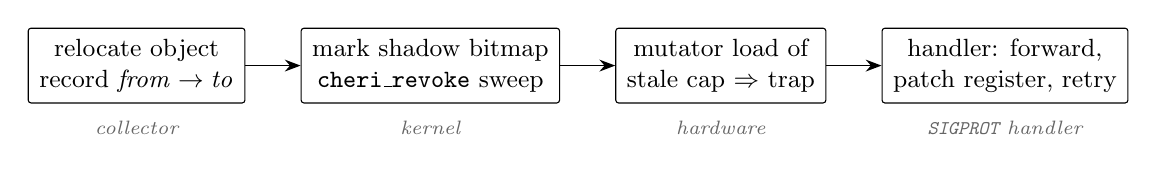
\begin{tikzpicture}[
  node distance=4mm and 7mm,
  box/.style={draw, rounded corners=1pt, align=center,
              font=\small, inner sep=4pt, minimum height=8.5mm},
  lbl/.style={font=\scriptsize\itshape, color=black!60},
  arr/.style={-{Stealth[length=2mm]}, semithick},
]
\node[box] (move)   {relocate object\\record $\mathit{from}\to\mathit{to}$};
\node[box, right=of move] (revoke) {mark shadow bitmap\\\texttt{cheri\_revoke} sweep};
\node[box, right=of revoke] (trap) {mutator load of\\stale cap $\Rightarrow$ trap};
\node[box, right=of trap] (heal) {handler: forward,\\patch register, retry};
\draw[arr] (move) -- (revoke);
\draw[arr] (revoke) -- (trap);
\draw[arr] (trap) -- (heal);
\node[lbl, below=1mm of move]   {collector};
\node[lbl, below=1mm of revoke] {kernel};
\node[lbl, below=1mm of trap]   {hardware};
\node[lbl, below=1mm of heal]   {\texttt{SIGPROT} handler};
\end{tikzpicture}
\caption{The trap--forward--resume protocol. The mutator's fast path
contains no barrier code: staleness detection is the capability tag
check the load--store unit performs on every purecap access anyway.}
\label{fig:protocol}
\end{figure}

\subsection{Overview}

StoplessGC manages a single contiguous arena. Allocation derives a
tight-bounds capability for each object from the arena's root
capability (\texttt{csetbounds} to the object's exact size, software
permissions stripped). A collection cycle (Figure~\ref{fig:protocol}):

\begin{enumerate}
\item \textbf{Relocate.} At a safepoint, scan the strong roots (thread
  stacks, OopStorage, class-loader data). Each root's referent is
  copied to a fresh arena slot with a capability-preserving copy (the
  copy must use capability loads/stores, or every reference field in
  the object loses its tag), the pair $(\mathit{from},\mathit{to})$ is
  recorded in the forwarding table, and the root slot is updated.
\item \textbf{Revoke.} The old object ranges are marked in the
  CheriBSD revocation shadow bitmap and a \texttt{cheri\_revoke} sweep
  is issued. After the sweep, every surviving capability to an old
  copy---heap fields, VM-internal slots, registers---is invalid.
\item \textbf{Heal lazily.} When a mutator dereferences a stale
  reference, the access traps (\texttt{SIGPROT}). The handler extracts
  the faulting capability from the saved register file, looks up its
  \emph{base address} in the forwarding table, rebuilds a valid
  capability to the new copy, writes it back to the faulting register,
  and returns; the instruction retries and succeeds. References that
  are never used are never healed and cost nothing.
\end{enumerate}

The protocol is self-correcting in the same sense as ZGC's self-healing
barrier: each stale reference traps at most a handful of times (once
per register copy) before the healed value propagates.

\subsection{The forwarding table must not contain capabilities}
\label{sec:design:fwd}

The single most consequential design point is what the forwarding table
stores. The obvious representation---map \texttt{from\_addr} to a
capability for the new object---is wrong, and fails in a way specific
to capability hardware.

The revocation sweep scans \emph{all} of memory, including the
collector's own metadata. Suppose object $A$ is moved to $A'$ in cycle
$i$ (table entry $A \to \mathrm{cap}(A')$), and $A'$ is itself moved in
a later cycle $j$ and its range revoked. The sweep finds the capability
$\mathrm{cap}(A')$ \emph{inside the forwarding table} and clears its
tag. A mutator that still holds a stale reference to $A$ then traps,
the handler looks up $A$---and hands back an untagged capability. The
mutator faults again, this time unforwardably. The failure is
non-deterministic (it needs an object to move twice with a live stale
reference across both moves) and presents as inexplicable corruption at
the start of unrelated cycles; disabling revocation makes it vanish,
which falsely implicates the sweep itself.

The fix follows from the diagnosis: store plain integers---destination
address and length---which the sweep cannot touch, and rebuild the
capability at lookup time from the arena's root capability:
\texttt{csetbounds(csetaddr(arena\_root, addr), len)}, with software
permissions stripped. Two details are load-bearing. First, the arena
root carries CheriBSD's \texttt{SW\_VMEM} software permission, which
exempts it from revocation, so the rebuild source survives every sweep.
Second, the rebuilt capability must reproduce the allocator's
\emph{exact tight bounds}: both the interior-pointer heal and the
identity barrier (below) key their lookups on
$\texttt{cheri\_base}(c)$, the object's base address. An early version
that rebuilt arena-wide capabilities broke reference identity in
\texttt{java.lang.invoke}'s identity-keyed caches, far from the
collector. The general law: \emph{on revocation-based systems, GC
metadata that must survive revocation must be integers, with
capabilities re-derived on demand from a revocation-exempt root.}

Forwarding entries persist across cycles, so a reference that is
multiple relocations stale heals through a chain of faults, one per
generation.

\subsection{The heal handler}
\label{sec:design:heal}

The handler receives the kernel's capability-fault signal and must
decide: stale (forward it) or genuinely bad (a real bug; re-raise). The
forwarding table itself is the oracle---only addresses the collector
relocated are in it. Three mechanics matter:

\begin{itemize}
\item \textbf{Register identification.} CheriBSD delivers the faulting
  PC, not the faulting capability. The handler scans the saved
  capability register file for registers that are untagged (or
  permission-stripped---CheriBSD kernels represent revocation either
  way, and the handler must accept both) and whose address forwards.
\item \textbf{Interior pointers.} A faulting capability may address a
  field or array element. Because allocation bounds are tight, the
  object's base is $\texttt{cheri\_base}$ of the faulting capability;
  the handler looks up the base and re-applies the offset to the
  rebuilt capability.
\item \textbf{Coexistence with expected faults.} HotSpot deliberately
  takes faults (the \texttt{SafeFetch} probes); on purecap these arrive
  as capability faults too, and every handler in the chain---including
  crash dumpers---must replay that redirect before treating a fault as
  fatal, and must itself attempt the heal path.
\end{itemize}

\subsection{The identity barrier}
\label{sec:design:acmp}

Reference equality (\texttt{if\_acmpeq/ne}, \texttt{==}) is the one
operation that observes addresses without dereferencing, so the
hardware barrier never fires: comparing a stale capability to a healed
one yields \emph{false} for the same object. ZGC solves this in the
load barrier (references are healed before comparison); we must solve
it at the comparison. The interpreter's compare becomes three-tier:
(1)~equal addresses $\Rightarrow$ equal (no relocation can make two
objects share an address); (2)~both capabilities tagged $\Rightarrow$
plain comparison is correct (neither is stale, because revocation
untags); (3)~otherwise, call a runtime that normalises both operands
through the forwarding table and compares the results. The fast paths
add two \texttt{gctag} instructions and a branch to one bytecode; the
slow path is rare (\S\ref{sec:eval:acmp}).

\subsection{Batched revocation}
\label{sec:design:batch}

The revocation sweep visits all mapped memory regardless of how many
objects are marked: revoking one object costs the same as revoking a
thousand. The shadow bitmap accumulates marks, and forwarding entries
already persist and chain across cycles. So the collector can relocate
every cycle but sweep every $N$th cycle, amortising the dominant cost
by up to $N$. The trade-off is a longer window in which old copies
remain dereferenceable: a not-yet-healed reference can read a stale
copy after the object has moved, which is correct only while relocation
is stop-the-world or objects are immutable in the window. A production
design would close the window with Morello's per-page capability-load
generation barrier, exactly as Cornucopia
Reloaded~\cite{cornucopia-reloaded} does for free--reuse windows; we
measure the amortisation (\S\ref{sec:eval:batch}) and leave the
load-barrier integration as future work.

% =====================================================================
\section{Implementation}
\label{sec:impl}

StoplessGC is implemented against OpenJDK~17 (jdk17u) on purecap
CheriBSD~15 (\texttt{aarch64c}). The collector proper is a CHERI-side
runtime library ($\sim$1.6\,kLOC of C: forwarding table, revocation
glue, signal handler) plus a HotSpot \texttt{CollectedHeap}
implementation ($\sim$1\,kLOC of C++: arena, root-scan closures, the
collection \texttt{VM\_Operation}, an optional concurrent collector
thread). Around 170 further patches against HotSpot make the template
interpreter and runtime capability-clean; they are mechanical but
load-bearing, and their failure modes are instructive. The classes that
cost the most time:

\begin{description}
\item[A64/C64 interworking.] Morello executes in two instruction-set
  modes; purecap code runs in C64. An indirect call through an
  \emph{integer} register (\texttt{blr x$n$} rather than
  \texttt{blr c$n$}) does not switch mode, and---the trap within the
  trap---setting the link address's low bit does \emph{not} set
  \texttt{PSTATE.C64}: the callee then decodes C64 prologue bytes as
  A64 garbage. Every interpreter codelet that calls into the VM through
  a raw function address had to be routed through capability branches.
\item[Capability-blind code generation.] Patterns that are correct on
  aarch64 silently strip tags on Morello: a conditional select
  (\texttt{csel}) on what is actually a capability value, integer
  compare-and-move on 16-byte object headers, an integer store
  overwriting half a capability. The 16-byte mark word also forces the
  header lock CAS to be a capability-sized CAS.
\item[DDC-relative assembly.] In purecap CheriBSD the default data
  capability is null; hand-written \texttt{.S} code that addresses
  memory as \texttt{[x0]} (DDC-relative) faults even though the
  ``pointer'' is valid. HotSpot's \texttt{SafeFetch} stubs were the
  prominent case.
\item[Signal-handler composition.] The GC trap handler, HotSpot's
  expected-fault machinery, and any diagnostic crash handler all
  receive the same signal; each must try \emph{all} the others'
  redirects (SafeFetch continuation, heal path) before declaring a
  fault fatal. Getting this wrong turns a healable stale-reference trap
  into a VM abort that looks like GC corruption.
\item[VM-internal raw references.] HotSpot's C++ code caches object
  addresses in places the root scan does not cover (interned handles,
  scratch fields). These never fault when merely \emph{copied} as
  values---only dereferences trap---so a stale cached reference can be
  compared, hashed, or stored long before the barrier can intervene.
  We bisected aggressive-relocation boot failures to this class
  (\S\ref{sec:limits}); it is the purecap analogue of the classic
  ``unreported root'' GC bug, made subtler because reads-as-values
  escape the hardware check.
\end{description}

The collection cycle itself runs as a safepoint \texttt{VM\_Operation};
an optional concurrent thread triggers cycles on a timer and is stable
under light load (\S\ref{sec:limits}). Relocation volume per cycle is
capped by a tunable move limit; integrity tests also run with the limit
effectively removed (every reachable root referent relocated,
1{,}016~objects in our largest configuration) to validate whole-heap
movement with correct reference identity.

% =====================================================================
\section{Evaluation}
\label{sec:eval}

\subsection{Setup and method}
\label{sec:eval:setup}

All measurements run on purecap CheriBSD~15.0-CURRENT
(\texttt{GENERIC-MORELLO-PURECAP}, \texttt{aarch64c}) under QEMU
system-mode emulation of Morello, with the OpenJDK~17 template
interpreter (\texttt{-Xint}), compressed oops and compressed class
pointers disabled, and the concurrent collector triggering cycles every
50\,ms with a per-cycle move limit of 8 objects unless stated. Phase
timings are taken inside the safepoint operation with the VM's
nanosecond clock, so the reported windows are exactly the mutator
pause; barrier-side counters (heal faults, heal time, identity
slow-path executions) are accumulated in the signal handler with a
monotonic clock and reported at VM exit.

\emph{What emulation does and does not invalidate.} QEMU inflates all
absolute times and does not model Morello's microarchitecture, so we
make no absolute-latency claims. The claims we do make are structural:
\emph{which} costs scale with \emph{what} (heap size, root count, batch
size), and those relationships are properties of the algorithm and the
revocation mechanism, not of the emulator. Workloads are purpose-built:
an allocation-heavy benchmark whose live set grows continuously
(\textsf{StoplessBench}), a linked-structure integrity test that
relocates every object and then verifies structure and reference
identity (\textsf{IntegrityGC}), and a string-concatenation workload
that exercises \texttt{invokedynamic}, \texttt{MethodHandle}
bootstraps, and identity-keyed caches (\textsf{ConcatTest}). They are
microbenchmarks, not DaCapo; running standard suites requires JIT and
library coverage beyond any current purecap JVM, including ours.

\subsection{The relocation pause is independent of heap size}
\label{sec:eval:flat}

\begin{figure}
\centering
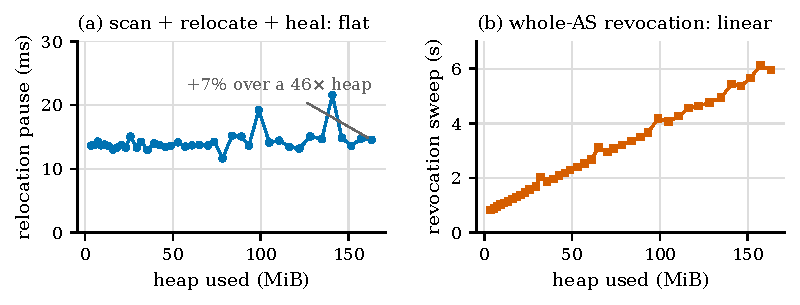
\includegraphics[width=\linewidth]{figs/heap_independence.pdf}
\caption{\textsf{StoplessBench}, root set constant at 894 after warm-up,
live heap growing $3.6\to163$\,MiB ($46\times$); 40 collection cycles,
8 objects relocated per cycle. (a)~The mutator-visible relocation phase
(root scan + copy + root fixup) stays at 13--15\,ms. (b)~The
\texttt{cheri\_revoke} sweep grows linearly with mapped memory,
$0.83\to5.95$\,s. Absolute times are QEMU-inflated; the claim is the
contrast in shape.}
\label{fig:flat}
\end{figure}

Figure~\ref{fig:flat} is the central result. \textsf{StoplessBench}
grows its live heap continuously while its root-set size stabilises,
isolating heap size as the variable. Over a $46\times$ heap range at a
constant 894 roots, the relocation pause moves from 13.7\,ms to
14.6\,ms ($+6\%$, within cycle-to-cycle noise), because the pause does
work proportional to roots scanned plus objects moved---never to heap
size. There is no marking phase, no per-object liveness traversal, and
no card or remembered-set scan in the pause: unreferenced old copies
are simply never healed, and their reclamation is the (off-pause)
revocation sweep. By contrast the sweep itself, panel~(b), is linear in
mapped memory---$0.83$\,s at $3.6$\,MiB to $5.95$\,s at
$163$\,MiB---confirming that sweeping, exactly as in the C/C++
revocation literature~\cite{cherivoke,cornucopia-reloaded}, is the cost
to engineer around, and motivating \S\ref{sec:eval:batch}.

\subsection{Cost of the barrier mechanisms}
\label{sec:eval:costs}

\begin{table}
\caption{Measured costs of the three mechanisms (QEMU-emulated;
relative magnitudes are the claim). Heal statistics from
\textsf{IntegrityGC} and \textsf{ConcatTest} under the concurrent
collector.}
\label{tab:triad}
\small
\begin{tabular}{llll}
\toprule
mechanism & cost & scales with & frequency \\
\midrule
relocation pause & 13--15\,ms & roots + moved objects & per cycle \\
revocation sweep & 0.83--5.95\,s & mapped memory & per cycle (or batch) \\
heal trap & 7--9\,\textmu s & --- & per \emph{used} stale ref \\
identity slow path & 2 table lookups & --- & 218 / run (\textsf{ConcatTest}) \\
\bottomrule
\end{tabular}
\end{table}

Table~\ref{tab:triad} summarises. Healing a trapped stale reference
---signal delivery, register-file scan, forwarding lookup, capability
rebuild, return-and-retry---averages 8.7\,\textmu s over 805 heals in
\textsf{IntegrityGC} and 7.0\,\textmu s over 903 heals in
\textsf{ConcatTest}; signal delivery dominates under emulation.
Aggregate heal time is $\sim$7\,ms per run---three orders of magnitude
below a single sweep---supporting the design's bet that lazy,
per-used-reference healing is cheap. The mutator's load fast path, to
restate, contains no added instructions at all.

\subsection{Batched revocation amortises the dominant cost}
\label{sec:eval:batch}

\begin{figure}
\centering
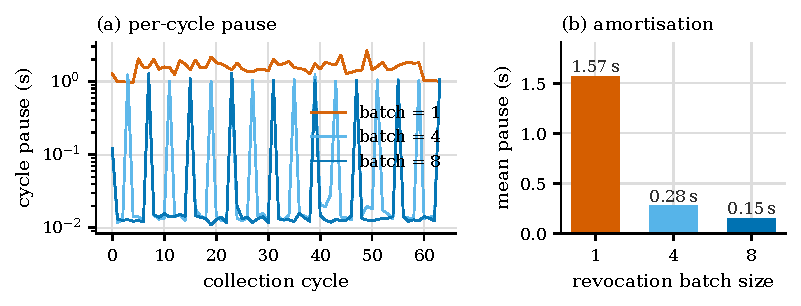
\includegraphics[width=\linewidth]{figs/batched_revoke.pdf}
\caption{Batched revocation, \textsf{IntegrityGC} under the concurrent
collector. (a)~Per-cycle pause, log scale: with batching most cycles
pause only for relocation ($\sim$15--25\,ms); the sweep cost
concentrates in every $N$th cycle. (b)~Mean pause per cycle falls from
0.84\,s to 0.07\,s ($11.9\times$) at batch size 32. The integrity test
passes at every batch size.}
\label{fig:batch}
\end{figure}

Because the sweep visits all memory regardless of marks, sweeping every
$N$th cycle divides its amortised cost by $N$ while relocation
continues every cycle. Figure~\ref{fig:batch}: mean pause per cycle
falls $0.843 \to 0.149 \to 0.071$\,s for batch sizes 1, 8, 32---a
$11.9\times$ reduction, tracking the sweep-count reduction
(62/23/4 sweeps over the respective runs)---and the structure-and-identity
verification passes at every batch size. The per-cycle trace shows the
expected shape: a floor at the heap-independent relocation pause, with
the sweep concentrated in periodic spikes whose amplitude is unchanged
(the sweep is no more expensive for being batched---that is the point).
The consistency caveat of \S\ref{sec:design:batch} applies: our
integrity tests do not mutate relocated objects inside the batch
window, and closing that window in general requires the per-page
load-barrier integration.

\subsection{The identity barrier is nearly free}
\label{sec:eval:acmp}

Over a full \textsf{ConcatTest} run---chosen because
\texttt{java.lang.invoke} bootstrap is dense with identity-keyed
caching---the identity barrier's slow path executed 218 times, against
903 heal faults and on the order of $10^6$ executed branches of the
fast path. Two extra tag-check instructions on a taken
\texttt{if\_acmp} bytecode, with table lookups only when an untagged
capability actually reaches a comparison, leaves reference equality
effectively unburdened.

% =====================================================================
\section{Discussion and limitations}
\label{sec:limits}

\paragraph{Emulation.} We re-emphasise: all absolutes are QEMU-scaled.
On hardware, signal delivery, memory bandwidth (the sweep is
bandwidth-bound~\cite{cherivoke}), and the relocation copy all shrink
by different factors; the flat-versus-linear contrast and the batching
arithmetic are preserved because they are counting arguments, not
timings. Reproducing Figure~\ref{fig:flat} on a Morello board is the
natural next step.

\paragraph{Stop-the-world relocation.} The measured configuration
relocates at safepoints; concurrency in StoplessGC currently means the
\emph{collector schedule} (a background thread triggering cycles, the
mutator running between them, healing on demand). True concurrent
relocation---mutators running \emph{during} the copy---needs an
object-granularity copy protocol; the hardware trap handles the
post-move window already, and revocation's atomic global cut-over is
precisely the property that makes the post-copy side tractable.

\paragraph{Coverage of VM-internal references.} Our root scan covers
the standard strong-root sets. HotSpot additionally caches raw object
addresses in VM-internal C++ state that is invisible to the root scan
and---because capability \emph{reads} do not trap, only
dereferences---can launder a stale reference back into circulation. We
hit this as boot-time failures under aggressive relocation and bisected
it to specific unscanned caches. The fix is the classic one (enumerate
or eliminate the caches); we flag it because the hardware barrier's
guarantee is easily over-read: it covers \emph{dereference}, not
\emph{data flow}.

\paragraph{Interpreter only.} Like all current purecap JVM work to our
knowledge~\cite{mojo-jvm,cheri-interpreter}, we run interpreted.
Template-interpreter bytecodes are exactly where our barrier costs sit
(the \texttt{acmp} tiers), so JIT changes the constant factors, not the
structure.

\paragraph{Memory overhead.} Old copies occupy arena space until swept,
so batching trades pause time for float, bounded by (moved bytes per
cycle)\,$\times$\,$N$; the forwarding table is three machine words per
relocated object per generation.

% =====================================================================
\section{Related work}
\label{sec:related}

\paragraph{CHERI revocation.} CHERIvoke~\cite{cherivoke},
Cornucopia~\cite{cornucopia}, and Cornucopia
Reloaded~\cite{cornucopia-reloaded} build and optimise sweeping
revocation for C/C++ temporal safety; revoked references are
use-after-free errors, terminal by design. We inherit their mechanism
(quarantine, shadow bitmap, sweep) and invert the trap's meaning, from
verdict to redirect. Cornucopia Reloaded's per-page load barrier is
also the missing piece for closing our batching window, a reunion of
the two lines we find pleasing.

\paragraph{Hardware-assisted read barriers.}
Appel--Ellis--Li~\cite{appel-ellis-li} used page protection as the
barrier; its page granularity caused multi-object stalls and its
protection flips are TLB-expensive. Capability revocation gives
\emph{per-object} (indeed per-capability) granularity with one global
cut-over. Azul Vega~\cite{pauseless} put the barrier in a custom
instruction, achieving per-reference granularity at the price of
bespoke silicon; CHERI offers the trap-on-stale primitive in a
general-purpose, security-motivated architecture.

\paragraph{Software barriers in production JVMs.}
ZGC~\cite{zgc-toplas,genzgc} and Shenandoah~\cite{shenandoah}
demonstrate that software self-healing barriers can reach
sub-millisecond pauses on commodity hardware, at a per-load
instruction cost and, for ZGC, a pointer encoding that purecap
disallows outright (\S\ref{sec:bg:zgc}). C4~\cite{c4} likewise relies
on address-space tricks (virtual-memory remapping) that capability
bounds constrain. Our contribution is not to outperform these
collectors but to show the barrier they implement in software is
already present, exact, and free-per-load in capability hardware.

\paragraph{Java on CHERI.} MOJO~\cite{mojo-jvm} ports OpenJDK~17's
Epsilon, Serial, and G1 to CheriBSD/Morello; Lowther et
al.~\cite{cheri-interpreter} optimise a MicroPython interpreter on
Morello. Neither moves objects under a hardware barrier.
Bramley et al.~\cite{cheri-allocators} study CHERI
\texttt{malloc} implementations, the non-moving end of the same design
space.

% =====================================================================
\section{Conclusion}
\label{sec:conc}

Capability revocation was built to make dangling pointers trap. A
moving garbage collector needs exactly that trap---plus a forwarding
table on the other side of it. StoplessGC demonstrates the
combination end to end in OpenJDK on Morello: relocation pauses bound
by roots rather than heap ($+6\%$ pause across a $46\times$ heap),
lazy per-use healing measured in microseconds, an identity barrier
that almost never takes its slow path, and a sweep cost that batches
away $11.9\times$ because revoking $n$ objects costs the same as
revoking one. The capability-specific lessons---integer-only GC
metadata rebuilt from revocation-exempt roots, identity as the one
barrier hardware cannot give you, reads-as-values as the residual
coverage gap---are, we believe, durable properties of building moving
collectors on this class of hardware, and the remaining engineering
(per-page load barriers for the batch window, concurrent copy, JIT) has
known designs waiting on the same substrate.

% =====================================================================
\paragraph{AI contribution statement.}
The design, implementation, debugging, measurement, and manuscript of
this work were produced by Claude (Anthropic)---Opus~4.8 and Fable~5
models, operating via Claude Code---under the direction, constraint
setting, and review of the human author. The division of labour is
recorded in the project repository's development log. Per current arXiv
and publisher policies, AI systems are not listed as authors because
authorship carries accountability; the human author assumes that
accountability and verified the empirical results and every citation.

\bibliographystyle{ACM-Reference-Format}
\bibliography{refs}

\end{document}
